%\documentclass{exam}
%\usepackage{enumitem}
%\usepackage{array}
%\usepackage{amsmath}
%\usepackage{float}
%\usepackage{graphicx}
%\begin{document}
\begin{enumerate}
	\item Solve the equations $x+2y=6$ and $2x-5y=12$ graphically.
	\vspace{4mm}
\item Solve the following equations for $x$ and $y$ using cross-multiplication method:\\
	\indent\indent\indent$(ax-by)+(a+4b)=0$\\\indent\indent$(bx+ay)+(b-4a)=0$
		\vspace{4mm}
\item Find the co-ordinates of the point where the line $\dfrac{x-3}{-1}=\dfrac{y+4}{1}=\dfrac{z+5}{6}$ crosses the plane passing through the points $\left(\dfrac{7}{2},0,0\right),(0,7,0),(0,0,7)$.
	\vspace{4mm}
\item Electrical transmission wires which are laid down in winters are stretched tightly to accommodate expansion in summers.\\
	\begin{figure}[H]
		\centering
		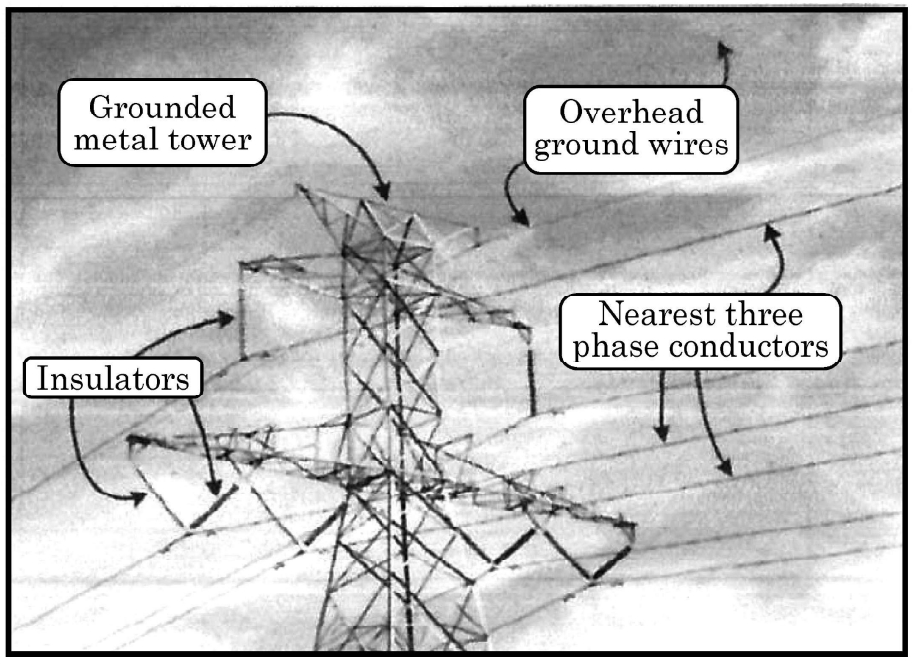
\includegraphics[height=5.5cm]{txn}\\
	\end{figure}
	Two such wires lie along the following lines:
\vspace{2.4mm}\\
	{\itshape\rmfamily $l_1$ : }$\dfrac{x+1}{3}=\dfrac{y-3}{-2}=\dfrac{z+2}{-1}$\vspace{1.35mm}\\
	{\itshape\rmfamily $l_2$ : }$\dfrac{x}{-1}=\dfrac{y-7}{3}=\dfrac{z+7}{-2}$\vspace{4.7mm}\\
	Based on the given information, answer the following questions:
		%\begin{parts}
		 %    \part
			\begin{enumerate}
				\item	Are the lines {\itshape\rmfamily $l_1$} and {\itshape\rmfamily $l_2$} coplanar? Justify your answer.
		 %\part
				\item    Find the point of intersection of lines {\itshape\rmfamily $l_1$} and {\itshape\rmfamily $l_2$.}
			\end{enumerate}
			%\end{parts}
		\vspace{4mm}
     \item Write the cartesian equation of the line PQ\@ passing through points P$(2,2,1)$ and Q$(5,1,-2)$. Hence, find the y-coordinate of the point on the line PQ whose z-coordinate is -2. 
				\vspace{4mm}
			\item Find the distance between the lines $x=\dfrac{y-1}{2}=\dfrac{z-2}{3}$ and $x+1=\dfrac{y+2}{2}=\dfrac{z-1}{3}$.
		\vspace{4mm}
\item Find the shortest distance between the following lines:
	\vspace{2mm}\\
	$\overrightarrow{\textbf{r}}=3\hat{i}+5\hat{j}+7\hat{k}+\lambda(\hat{i}-2\hat{j}+\hat{k})$ and $\overrightarrow{\textbf{r}}=(-\hat{i}-\hat{j}-\hat{k})+\mu(7\hat{i}-6\hat{j}=\hat{k})$.
	\vspace{4mm}
\item Two motorcycles A and B are running at a speed more than the allowed speed on the roads represented by the lines $\overrightarrow{\textbf{r}}=\lambda(\hat{i}+2\hat{j}-\hat{k})$ and $\overrightarrow{\textbf{r}}=(3\hat{i}+3\hat{j})+\mu(2\hat{i}+\hat{j}+\hat{k})$ respectively.\\
	\begin{figure}[H]
		\centering
		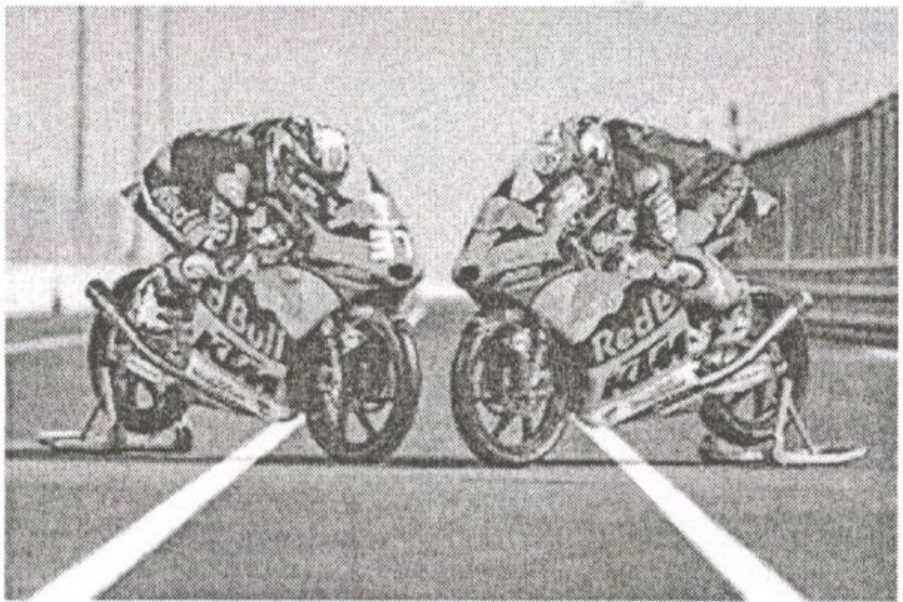
\includegraphics[height=5.5cm]{bike}\\
	\end{figure}
	Based on the following information, answer the following questions:
	\begin{enumerate}
		\item Find the shortest distance between the given lines.
		\item Find a point at which the motorcycles may collide.
	\end{enumerate}
	\vspace{4mm}
\item Find the shortest distance between the lines\\\vspace{2mm}
	$\overrightarrow{\textbf{r}}=(\lambda+1)\hat{i}+(\lambda+4)\hat{j}-(\lambda-3)\hat{k}$, and\\
			\vspace{2mm}$\overrightarrow{\textbf{r}}=(3-\mu)\hat{i}+(2\mu+2)\hat{j}+(\mu+6)\hat{k}$
			\vspace{4mm}
\item Find the shortest distance between the following lines and hence write whether the lines are intersecting or not.\vspace{2mm}\\
	$\dfrac{x-1}{2}=\dfrac{y+1}{3}=z$, $\dfrac{x+1}{5}=\dfrac{y-2}{1}$, $z=2$
\end{enumerate}
%\end{document}
